% Advanced NLP - Assignment 1 Report
% Formatting per the assignment brief: 12pt Times New Roman, 1-inch margins,
% maximum 6 pages excluding references and links.
%
% Compile from this directory (the figure paths are relative to it):
%   pdflatex Report.tex && pdflatex Report.tex
% Then copy Report.pdf into 2023111026_assignment1/.

\documentclass[12pt]{article}

\usepackage[margin=1in]{geometry}
\usepackage{mathptmx}          % Times New Roman for text and math
\usepackage[T1]{fontenc}
\usepackage[utf8]{inputenc}
\usepackage{graphicx}
\usepackage{booktabs}
\usepackage{array}
\usepackage{placeins}          % \FloatBarrier, to stop floats drifting past a section
\usepackage{titlesec}
\titlespacing*{\section}{0pt}{1.6ex plus .2ex}{0.8ex}
\titlespacing*{\subsection}{0pt}{1.3ex plus .2ex}{0.6ex}
\newcolumntype{R}[1]{>{\raggedright\arraybackslash}p{#1}}
\usepackage{amsmath}
\usepackage{caption}
\usepackage{xurl}              % allow long URLs to wrap inside the margins
\usepackage[hidelinks]{hyperref}

\captionsetup{font=small,labelfont=bf,skip=4pt}

% Allow a larger share of each page to be occupied by floats, so figures sit
% near the text that discusses them instead of drifting to the end.
\renewcommand{\topfraction}{0.95}
\renewcommand{\bottomfraction}{0.95}
\renewcommand{\textfraction}{0.05}
\renewcommand{\floatpagefraction}{0.8}
\setcounter{topnumber}{3}
\setcounter{bottomnumber}{2}
\setcounter{totalnumber}{5}
\setlength{\parskip}{0.15em}
\setlength{\parindent}{0pt}

\title{\vspace{-1.2cm}Advanced Natural Language Processing\\Assignment 1 Report}
\author{Arihant Tripathy\\\normalsize Roll number: 2023111026}
\date{}

\begin{document}
\maketitle
\vspace{-1cm}

\section{Preliminary Analysis}

The dataset consisted of 2 files, \texttt{brown\_plain.txt} and
\texttt{brown\_cipher.txt}, containing 5,000 lines each. I took the assumption
here that our goal is to train a model to decrypt the cipher text into plain
text.

My first step was to analyze the dataset.

The plain text file contained only upper and lower case letters, and spaces. The
cipher text file contained only 0s and 1s. There were no empty lines in either
file. Each line in the cipher file was 8 times the length of the same line in
the plain text file, which meant that each character in plain text was
represented by 8 bits in cipher text.

I found out that the encryption technique used was a repeating key XOR cipher
with the 8-character key \texttt{ANLP2026}. In this method, each plaintext
character is first converted into its ASCII value. The corresponding key
character is also converted into ASCII, and the two values are XORed. The result
is the encrypted byte for that character. Because the key has 8 characters, it
repeats throughout the whole line. This means the 1st character is XORed with
\texttt{A}, the 2nd with \texttt{N}, the 3rd with \texttt{L}, and so on. After
the 8th character, the same key pattern starts again from the beginning. The
encrypted value of each character is then written as an 8-bit binary number.
Decryption is done by XORing the encrypted byte with the same key character,
which gives back the original plaintext character.

\section{Training}

I split the dataset into training, validation, and test sets in the ratio
80:10:10. Then, I wrote the initial code for the transformer model, and started
training. I immediately encountered Out of Memory errors, and the training was
very slow too. This is because the longest line length in the dataset is 2,670
characters, and processing such long sequences required a lot of memory. So to
reduce memory usage, I decided to process the ciphertext in chunks rather than
full lines. Since the cipher uses an 8-character repeating key, the chunk size
was chosen as a multiple of 8 characters (256) so every chunk starts at the same
key phase, keeping the ciphertext-to-plaintext mapping consistent across
samples.

The total GPU training time across all five configurations was about 2 hours 49
minutes.

\subsection{Configurations}

For the first four configurations (C1--C4), I used a tokenized approach, where
the input was tokenized into 8-bit chunks. Each chunk was treated as a separate
token, with a token ID from 0 to 255. Since the window size is a multiple of 8,
every chunk starts at the same key phase. This causes the ciphertext-to-plaintext
mapping to be consistent across samples. For the fifth configuration (C5), I
used a token-free approach, where the input was processed as a sequence of bits,
and it outputs a sequence of raw plaintext bytes.

The common hyperparameters for all configurations were the following:

\begin{enumerate}\itemsep0pt
  \item Each token is represented as a 256-dimensional embedding vector
        (\texttt{d\_model = 256})
  \item 8 attention heads
  \item 4 encoder layers
  \item 4 decoder layers
  \item Feed forward dimension of 1024
  \item Dropout of 0.1
  \item AdamW optimizer with a learning rate of 3e-4, 1000 warmup steps, and
        cosine decay scheduler
  \item Label smoothing of 0.1 to prevent overfitting
  \item \texttt{bfloat16} autocast for faster training and lower memory usage
  \item Maximum epochs of 80, with early stopping if validation loss does not
        improve for 10 consecutive epochs
\end{enumerate}

The differences between the configurations were as follows:

\begin{table}[!htb]
\centering
\small
\setlength{\tabcolsep}{4pt}
\begin{tabular}{@{}lR{2.2cm}R{2.2cm}R{2.3cm}R{2.4cm}R{2.4cm}@{}}
\toprule
Config & Change from Base & Positional Encoding & Attention Mechanism &
Normalization & Tokenization \\
\midrule
C1 & None (Base) & Sinusoidal Absolute & Multi-Head Attention & LayerNorm &
Standard Subword \\
C2 & Positional encoding & \textbf{RoPE} & Multi-Head Attention & LayerNorm &
Standard Subword \\
C3 & Attention mechanism & Sinusoidal Absolute & \textbf{Grouped-Query} &
LayerNorm & Standard Subword \\
C4 & Normalization & Sinusoidal Absolute & Multi-Head Attention &
\textbf{RMSNorm} & Standard Subword \\
C5 & Tokenization & Sinusoidal Absolute & Multi-Head Attention & LayerNorm &
\textbf{BLT (Token-Free)} \\
\bottomrule
\end{tabular}
\caption{The five architectural configurations.}
\end{table}

\section{Results}

Test-set results for the five configurations. BLEU/ROUGE apply to tokenized
models only.

\begin{table}[!htb]
\centering
\small
\setlength{\tabcolsep}{5pt}
\begin{tabular}{@{}lrrrrrrr@{}}
\toprule
Config & Bit Acc. & Seq. Acc. & Levenshtein & BLEU & ROUGE-1 & ROUGE-2 &
ROUGE-L \\
\midrule
C1 (base)    & 0.720 & 0.004 & 54.50 & \textbf{67.12} & 0.818 & \textbf{0.702} & 0.817 \\
C2 (RoPE)    & 0.704 & 0.004 & 83.75 & 61.98 & 0.779 & 0.652 & 0.776 \\
C3 (GQA)     & 0.709 & 0.006 & 83.23 & 57.49 & 0.765 & 0.622 & 0.763 \\
C4 (RMSNorm) & 0.719 & 0.004 & 54.37 & 66.79 & \textbf{0.821} & \textbf{0.702} & \textbf{0.820} \\
C5 (BLT)     & \textbf{0.990} & \textbf{0.296} & \textbf{4.02} & -- & -- & -- & -- \\
\bottomrule
\end{tabular}
\caption{Test-set results for the five configurations.}
\end{table}

\begin{figure}[!htb]
\centering
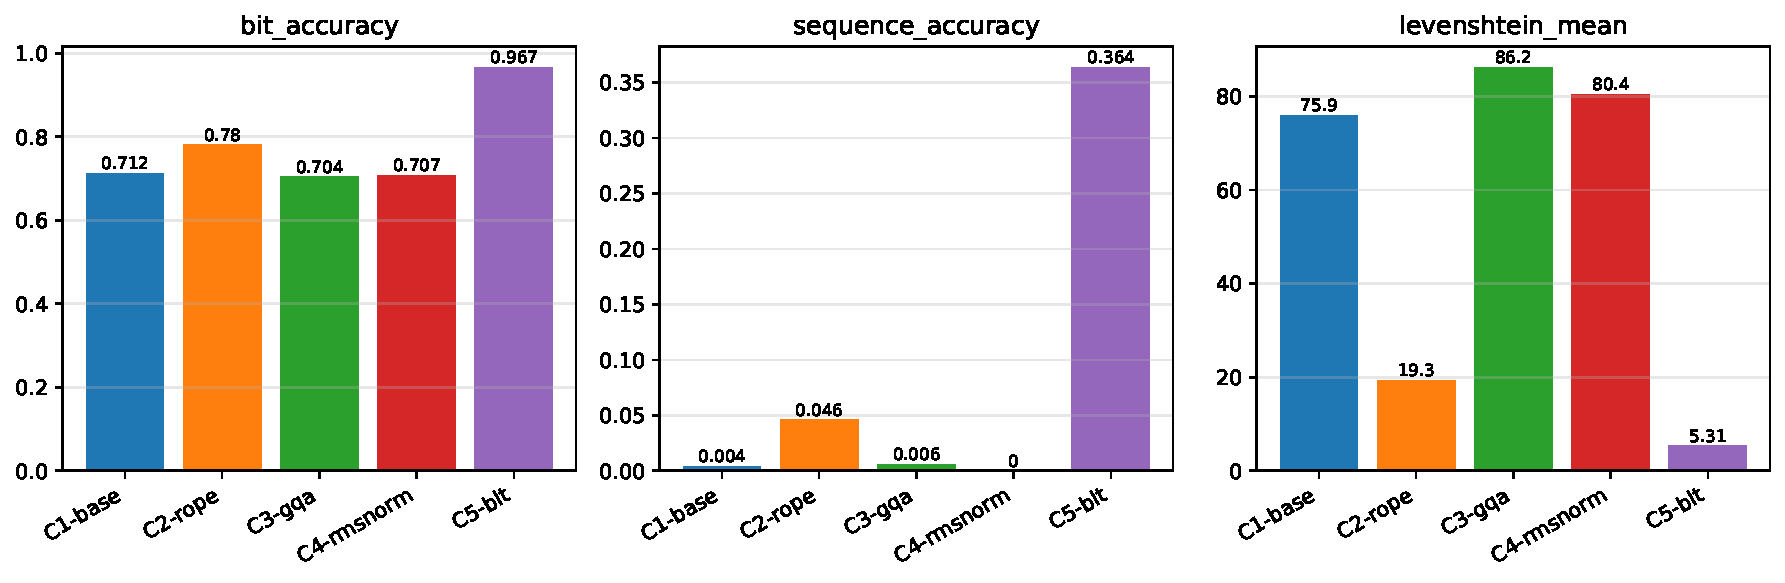
\includegraphics[width=0.8\linewidth]{../2023111026_assignment1/outputs/plots/metrics_all.pdf}
\caption{Overall test metrics across all five configurations.}
\end{figure}

\begin{figure}[!htb]
\centering
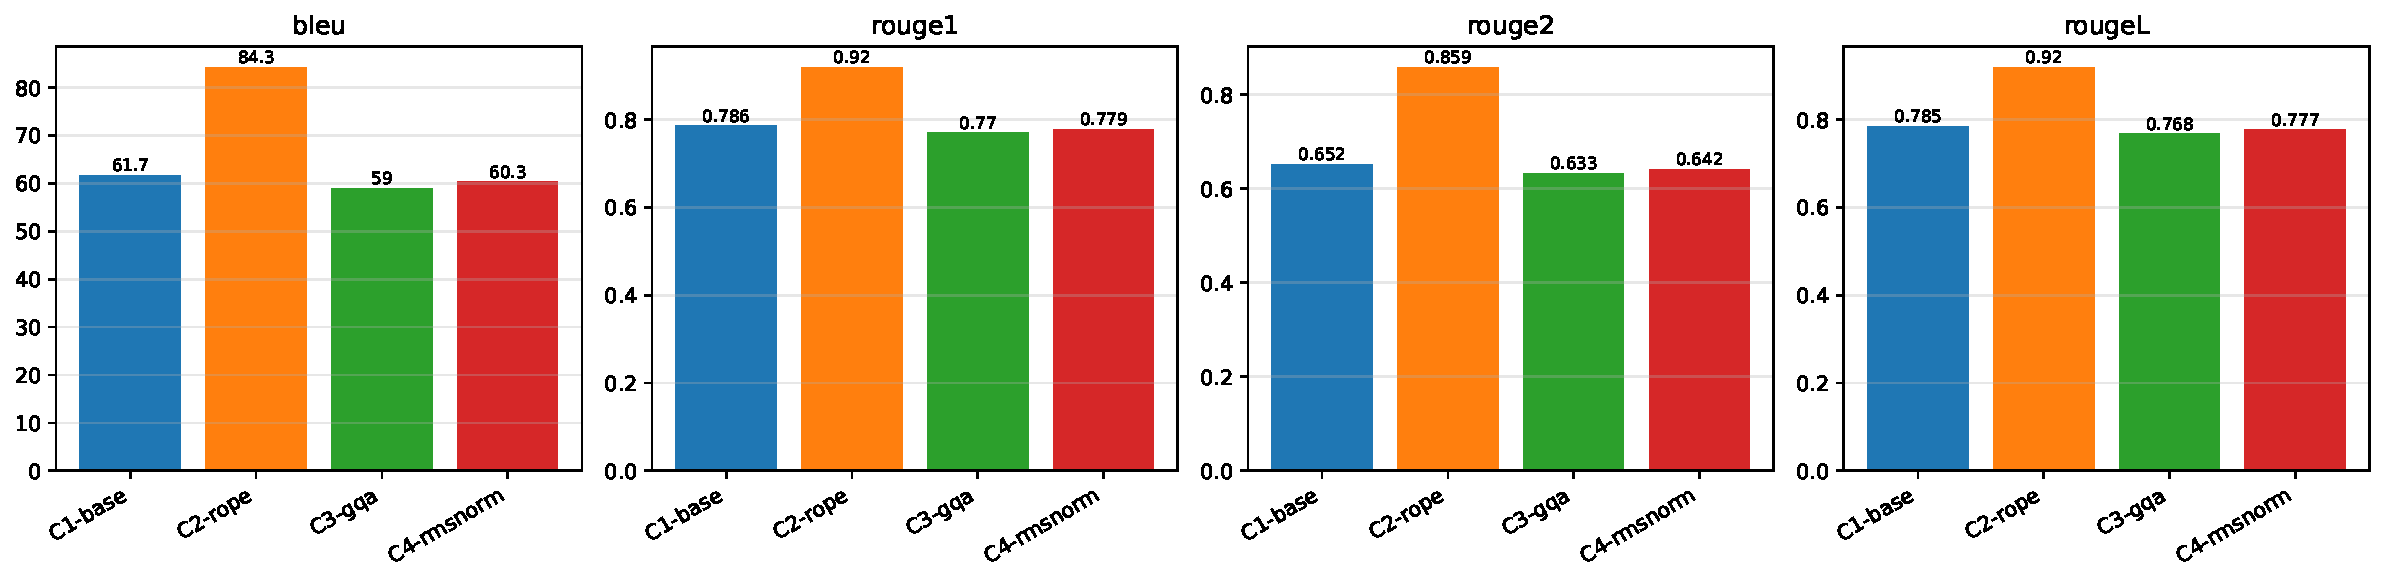
\includegraphics[width=0.8\linewidth]{../2023111026_assignment1/outputs/plots/metrics_bleu_rouge.pdf}
\caption{BLEU and ROUGE comparison for the tokenized configurations (C1--C4).}
\end{figure}

\begin{figure}[!htb]
\centering
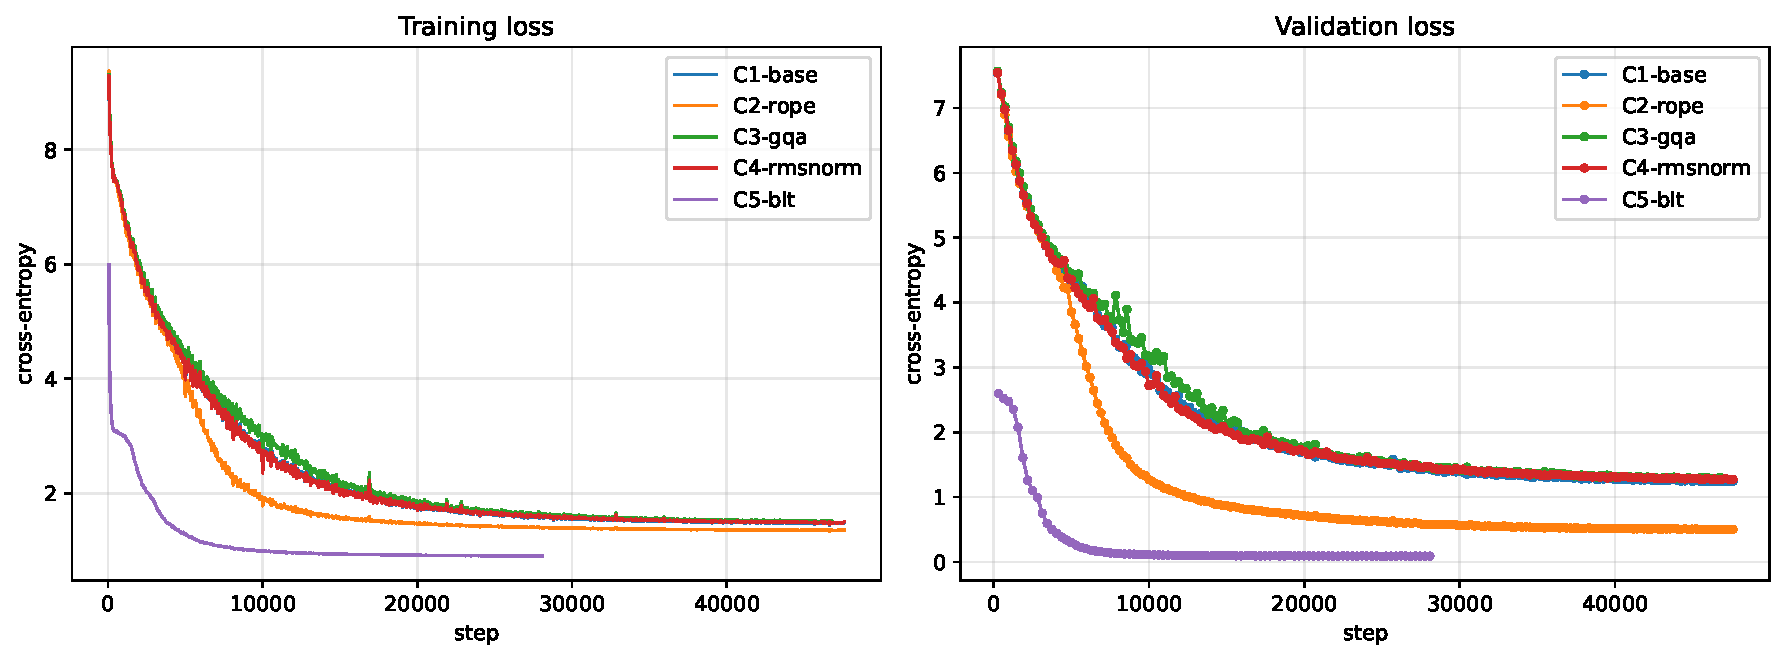
\includegraphics[width=0.8\linewidth]{../2023111026_assignment1/outputs/plots/loss_curves.pdf}
\caption{Training and validation loss for all configurations.}
\end{figure}

\subsection{C1: Baseline}

C1 is the baseline configuration, which uses sinusoidal absolute positional
encoding, multi-head attention, layer normalization, and standard subword
tokenization.

\subsection{C2: RoPE vs.\ sinusoidal absolute}

C2 replaces the sinusoidal absolute positional encoding with Rotary Positional
Encoding (RoPE). While normal positional encoding turns the input into a fixed
embedding, and adds another vector which represents the position of the token,
RoPE doesn't have a separate positional embedding. Instead, it rotates the query
and key vectors based on their position. This can help the model to better
capture relative positions between tokens, in theory.

However, in this case, the performance of C2 is worse than C1. The Bit Accuracy
drops from 0.720 to 0.704, while the Levenshtein Distance increases from 54.50
to 83.75. The BLEU score also drops from 67.12 to 61.98, and ROUGE scores
decrease as well. One possible reason is that RoPE is applied to the
self-attention blocks, while the cross-attention uses unrotated queries and
keys. The model needs to learn the exact positional mapping between the
ciphertext and plaintext, which is a cross-attention task. Therefore, absolute
positional encoding might be more suitable for this task.

\subsection{C3: Grouped-Query vs.\ Multi-Head Attention}

In MHA, each attention head has its own query, key, and value matrices. In GQA,
I split the 8 attention heads into 2 groups, so the 8 query heads share 2
key/value heads. Each key/value pair is shared across 4 query heads. This
reduces the key and value matrices from $256 \times 256$ to $256 \times 64$,
saving 98,304 weights and 384 bias terms per self-attention block. Across 8
blocks, this saves 789,504 parameters (8\%).

GQA is more useful in larger models, where the KV cache is big and can afford to
be reduced. In this case, the model is small, and the KV cache is already small,
so reducing it further hurts performance. The Bit Accuracy drops from 0.720 to
0.709, while the Levenshtein Distance increases from 54.50 to 83.23. It also has
the worst validation loss at 1.06, compared to the baseline's 0.81. The
reduction in self-attention capacity in GQA was harmful in this particular task,
where small positional and contextual differences are important.

\subsection{C4: RMSNorm vs.\ LayerNorm}

This configuration changes the normalization layer from LayerNorm to RMSNorm.
LayerNorm subtracts the mean, divides by the standard deviation, then scales and
shifts by learned parameters. In RMSNorm, only the root mean square (RMS) of the
input is calculated, and the input is normalized using it. This reduces the
number of parameters in each normalization layer from 512 to 256, saving 256
parameters per layer. The model has 22 normalization sites in total (2 per
encoder layer, 3 per decoder layer, and a final norm on each stack), so this
saves 5,632 parameters (0.06\%).

Consequently, the performance of C4 is very similar to C1, with a Bit Accuracy
of 0.719 (vs.\ 0.720) and Levenshtein Distance of 54.37 (vs.\ 54.50). The BLEU
score is 66.79 compared to the baseline's 67.12, and ROUGE scores are also very
close to C1, if not slightly better at times. RMSNorm was also the fastest
configuration to train, with a throughput of 486.3 samples/s, compared to C1's
474.6 samples/s. This shows that RMSNorm reduces the math operations required
for normalization, and hence speeds up training, while maintaining similar
performance to LayerNorm.

\subsection{C5: Token-free approach}

For this, I replaced the tokenizer with a Byte Latent Transformer (BLT). Instead
of converting groups of 8 bits into a single token, the BLT processes the
ciphertext as a sequence of individual binary values. Since processing all 2048
positions with unrestricted attention is very memory-intensive, I restricted the
local attention to 128-position windows. The resulting representations are then
grouped into sets of 8 consecutive values and compressed into patch
representations. Since 8 cipher bits represent one plaintext character, each
patch corresponds to one plaintext character. This reduces the sequence from
2048 positions to 256 patches before it reaches the global Transformer.

This approach performs much better than the tokenized configurations. It is able
to achieve a Bit Accuracy of 0.990 and a Sequence Accuracy of 0.296, compared to
0.720 and 0.004 for C1. The Levenshtein Distance is also much lower at 4.02,
compared to the baseline's 54.50. This is because the patching mechanism creates
a direct alignment between each group of 8 ciphertext bits and one plaintext
character.

However, C5 is more expensive to train. It has 12.51M parameters compared to
9.49M for C1, and its throughput is much lower at 120.7 samples/s compared to
474.6 samples/s. Its training time per epoch increases from 24.2 seconds to 95.1
seconds, while peak GPU memory increases from 3.15 GB to 6.06 GB. This overhead
comes mainly from processing the longer byte-level sequence in the local encoder
and decoder. One point to note is that C5 reached its best checkpoint at epoch
15, after about 24 minutes, and then stopped early at epoch 25 for a total of
about 40 minutes. C1's best checkpoint came from epoch 79, after about 32
minutes. So if we just care about the time to get the best model, C5 is actually
faster than C1.

\begin{table}[!htb]
\centering
\small
\begin{tabular}{@{}lrrrrr@{}}
\toprule
Config & Params & Samples/s & Tokens/s & s/epoch & Peak GPU mem (GB) \\
\midrule
C1 (base) & 9.49M  & 474.6 & 22729 & 24.2 & 3.15 \\
C5 (BLT)  & 12.51M & 120.7 & 25499 & 95.1 & 6.06 \\
\bottomrule
\end{tabular}
\caption{Training efficiency, C1 vs.\ C5.}
\end{table}

\begin{figure}[!htb]
\centering
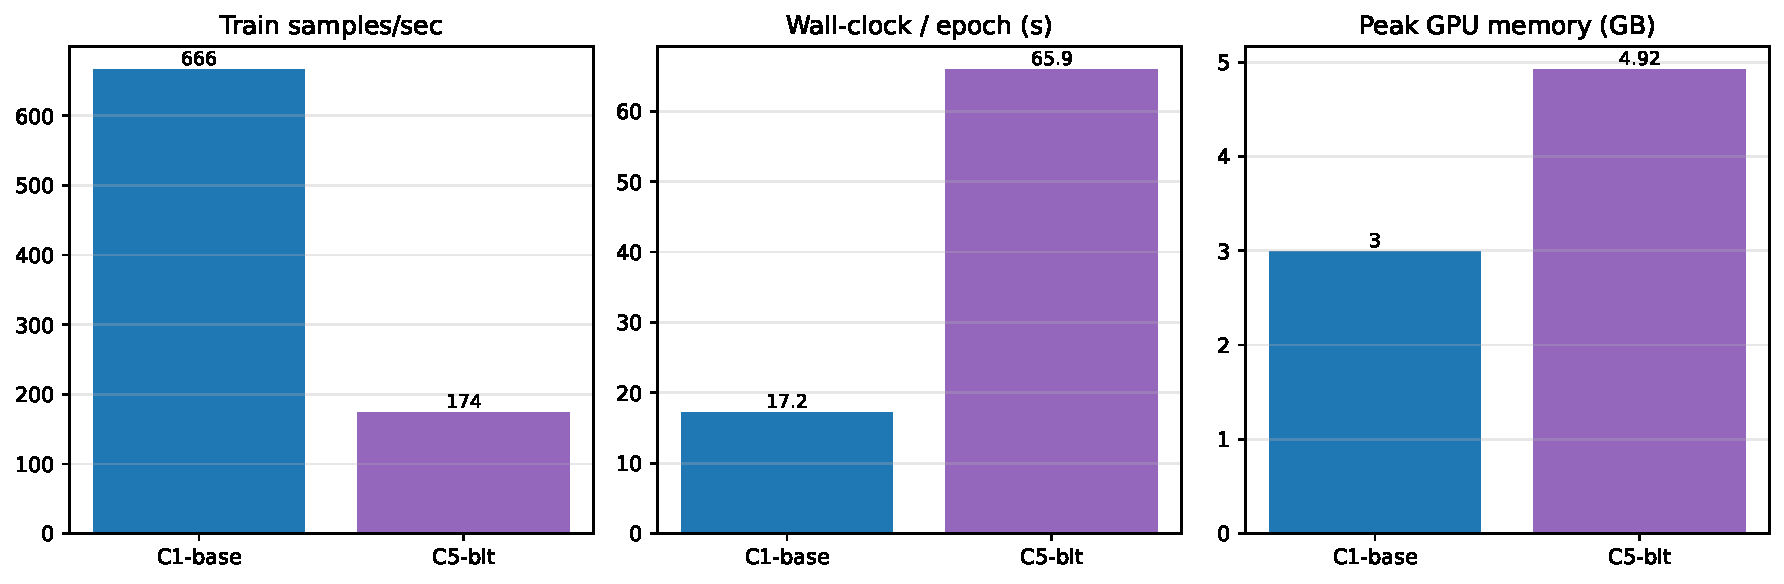
\includegraphics[width=0.78\linewidth]{../2023111026_assignment1/outputs/plots/c5_vs_c1_benchmark.pdf}
\caption{C1 vs.\ C5: throughput, wall-clock per epoch, and peak GPU memory.}
\end{figure}

\FloatBarrier
\section*{Links}

\begin{itemize}\itemsep0pt
  \item Weights \& Biases project:
        \url{https://wandb.ai/arihanttr-iiit-hyderabad/anlp-a1}
  \item Hugging Face checkpoints:
        \url{https://huggingface.co/Arihant25/anlp-a1-transformer-ablations}
\end{itemize}

\end{document}
